%Dies ist die Hauptseite des Dokumentes. Es werden u. a. alle Kapitel,
%Einstellung im Header eingebunden.  Veränderungen müssen in folgenden Dateien
%vorgenommen werden:
      %- einzelne Kapitel (evtl. erweitern)

% Declare document wide classes
\documentclass[
    11pt,                   % Default font size
  DIV12,
    oneside,                % One-sided document
    titlepage,              % Has a specific page for the title
    parskip=half,           % Spacing between paragraphs
    headings=normal,        % Smaller headings size
    captions=tableheading,
    final                   % Document is marked as final
]{scrreprt}               %

% Include the packages
% Do we need this?
\usepackage{fix-cm}


% Do we need this?
\usepackage[T1]{fontenc}
\usepackage{lmodern}
\usepackage[utf8]{inputenc}

% Setting language of babel to english
\usepackage[english]{babel}

% Helpers for geometry and spacing settings
\usepackage{geometry}
\usepackage{setspace}
\usepackage{float}

% Adapt font sizes for different sections
\usepackage{relsize}

% Lines in header and footer
\usepackage[headsepline, footsepline, ilines]{scrlayer-scrpage}

% Graphics and colors
\usepackage{xcolor}
\usepackage{graphicx}

% Hyphenation and underlining
\usepackage{soul}

% Additional font family
\usepackage{helvet}

\usepackage{appendix}
\usepackage{pdfpages}
\usepackage{float}

% Big tables
\usepackage{longtable}
\usepackage{array}
\usepackage{ragged2e}
\usepackage{lscape}

\usepackage[normalem]{ulem}

\usepackage{enumitem}

% For YAML-syntax highlighting
\usepackage{minted}

% Options for pdf generation
\usepackage[
  bookmarks,
  bookmarksopen=true,
  colorlinks=true,
  linkcolor=black,        % Links have black color
  anchorcolor=black,      % Links have black color
  citecolor=black,        % Links have black color
  filecolor=black,        % Links have black color
  menucolor=black,        % Links have black color
  urlcolor=black,         % Links have black color
  backref,                % Do we need this?
  pagebackref,            % Do we need this?
  plainpages=false,       % Allows setting bookmarks (Do we need ths?)
  pdfpagelabels,          % Allows setting bookmarks (Do we need ths?)
  hypertexnames=false,    % Allows setting bookmarks (Do we need ths?)
  linktocpage             % Link page numbers in table of contents
  ]{hyperref}

\usepackage{tabularx}
\usepackage{booktabs}
\usepackage{pifont}
\usepackage{float}


  \usepackage{verbatim}








% Geometric specific settings
\geometry{
    paper=a4paper,
    top=25mm,
    left=25mm,
    right=25mm,
    bottom=45mm,
    pdftex
  }

% Page layout
\onehalfspace        % 1.5x spacing

\pagestyle{scrheadings}

% Header and footer on new section pages
\renewcommand*{\chapterpagestyle}{scrheadings}

% Font size of headers
\renewcommand{\headfont}{\normalfont}

% Custom colors
\definecolor{tuRed}{cmyk}{1.0,0.0,0.6,0.0}

% Header config
\setheadsepline{1pt}[\color{tuRed}]
\setlength{\headheight}{21mm}        % Header height
\ihead{\large{\textsc{CodeX: Natural-Language to Structured Code Generation}}\\    % Text in left box
       \small{Requirements Analysis}}
\chead{}                            % Text in center box

% Footer config
\setfootsepline{1pt}[\color{tuRed}]
\cfoot{}                            % Text in center box
\ofoot{\pagemark}                    % Page counter in right box



% Custom definitions for refs with custom text
% Black magic. Don't touch, it will break
\makeatletter
\def\namedlabel#1#2{\begingroup
#2
\def\@currentlabel{#2}
\phantomsection\label{#1}\endgroup
}
\makeatother


% Utility command for setting a counter based on a ref
\newcommand{\refsetcounter}[2]{\setcounter{#1}{#2}\addtocounter{#1}{-1}\refstepcounter{#1}}

% Environment for product functions
\newcounter{functioncount} 
\newenvironment{function}[2]{\refsetcounter{functioncount}{#1}\large\textbf{\sffamily{#2 }}\namedlabel{F#1}{$\langle F#1\rangle$}\normalsize\begin{description}\setlength{\itemsep}{-5pt}}{\end{description}}

% Environment for data (what is this for?)
\newcounter{datacount} 
\newenvironment{data}[2]{\refsetcounter{datacount}{#1}\textbf{#2} \namedlabel{D#1}{$\langle D#1\rangle$}\\}{}

% Commands for criteria

\newcommand{\should}[1]{\textlangle RS#1\textrangle}
\newcommand{\must}[1]{\textlangle RM#1\textrangle}
\newcommand{\could}[1]{\textlangle RC#1\textrangle}

\newcommand{\prodFunc}[1]{\textlangle F#1\textrangle}
\newcommand{\test}[1]{\textlangle T#1\textrangle}

% Criteria command for wont-do-criteria
\newcommand{\wont}[2]{\refsetcounter{datacount}{#1}\namedlabel{RW#1}{$\langle RW#1\rangle$} #2\\}

% Criteria command for quality criteria
\newcommand{\qualityReq}[2]{\refsetcounter{datacount}{#1}\namedlabel{Q#1}{$\langle Q#1\rangle$} #2\\}

% Environment for ui (what is this for)?
\newcounter{uicount}
\newenvironment{ui}[2]{\refsetcounter{uicount}{#1}\textbf{#2} \namedlabel{UI#1}{$\langle UI#1\rangle$}\\}{}


% Environment for class (what is this for)?
\newcounter{classcount}
\newenvironment{class}[2]{\refsetcounter{classcount}{#1}\textbf{#2}\namedlabel{CL#1}{$\langle CL#1\rangle$}\begin{description}\setlength{\itemsep}{-5pt}}{\end{description}}

% Environment for entities (what is this for)?
\newcounter{entitycount}
\newenvironment{entity}[2]{\refsetcounter{entitycount}{#1}\textbf{#2} \namedlabel{E#1}{$\langle E#1\rangle$}\\}{}

% Environment for components (what is this for)?
\newcounter{componentcount}
\newenvironment{component}[2]{\refsetcounter{componentcount}{#1}\textbf{Component \namedlabel{C#1}{$\langle C#1\rangle$}: #2}\\}{}

% Environment for interface (what is this for)?
\newcounter{interfacecount}
\newenvironment{interface}[2]{\refsetcounter{interfacecount}{#1}\textbf{Schnittstelle \namedlabel{I#1}{$\langle I#1\rangle$}: #2}\\}{}

% Environment for testcase (what is this for)?
\newcounter{testcasecount}
\newenvironment{testcase}[2]{\refsetcounter{testcasecount}{#1}\textbf{Test-Case #2}\namedlabel{T#1}{$\langle T#1\rangle$}\normalsize\begin{description}\setlength{\itemsep}{-5pt}}{\end{description}\hspace{7.5em}}
           % Diese Datei enthält alle
                                           % Layouteinstellungen

\setcounter{secnumdepth}{3}

%------Beginn des Gesamtdokumentes----------------------------------------------
\begin{document}

%------Eingebundene Seiten, Verzeichnisse bzw. Kapitel--------------------------
% Header is empty for title page
\thispagestyle{plain}

% Begin of title page
\begin{titlepage}


\vspace*{-3.8cm}
\hspace*{-2cm}\begin{minipage}{1.25\textwidth}

\includegraphics[width=5.3cm]{common/kit_logo}\setlength{\unitlength}{1mm}\begin{picture}(00,00)(-10,0)\color{tuRed}\put(000,004){\line(1,0){140}}\end{picture}%\hfill
\parbox[b]{0.68\textwidth}{\hfill
\includegraphics[width=8cm,height=2.4cm,keepaspectratio]{common/cdnc_logo}\\~}
\end{minipage}

\hypersetup{
pdftitle={CodeX - Design},
pdfauthor={Oleksandr Brittner, Simon Bumiller, Simon Gaber, Dayana Karadzhova, Kyrylo Pavlov}
}

~\\[5ex]

% Center everything on the title page
\begin{center}
% Title of module
{\relsize{4}{\textbf{\textsc{CodeX: Natural-Language to Structured Code Generation}}}}\\[5ex]

{\relsize{3}{\textbf{Implementation}}}\\[5ex]

Winter Term 2025/2026\\[6ex]


% Institution
Karlsruhe Institute of Technology (KIT)\\
ITEC - Institute of Computer Engineering\\
Chair of Dependable Nano Computing

~\\[2ex]

\begin{tabular}{c c c}
    Oleksandr Brittner & Simon Bumiller & Simon Gaber \\
    ugzsu@student.kit.edu & ugpiq@student.kit.edu & upiko@student.kit.edu
\end{tabular}


~\\[1ex]

\begin{tabular}{c c}
    Dayana Karadzhova & Kyrylo Pavlov\\
    utguc@student.kit.edu & uxrnz@student.kit.edu
\end{tabular}

\vspace{5.0em}

\textbf{Supervised by:}
\begin{tabular}{c c}
    Haneen Gamal Mohamed Hezayyin Seyam & Maha Elsayed Mohamed Shatta \\
    haneen.seyam@kit.edu & maha.shatta@kit.edu
\end{tabular}

% City, Date
\vfill
Karlsruhe, \today

\end{center}
\end{titlepage}

{\relsize{3}{\textbf{Contribution}}}\\[5ex]

\begin{tabular}{p{9cm}p{7cm}}
Implementation Status & Simon Bumiller \\[0.4em]


Working Methodology and Approach & Dayana Karadzhova \\[0.4em]
Schedule and Timeline Analysis & Dayana Karadzhova \\[0.4em]
Internal Communication & Dayana Karadzhova \\[0.4em]
Technical Development Environment & Dayana Karadzhova \\[0.4em]
Version Control and Workflow & Dayana Karadzhova \\[0.4em]

Deviations from the Design Document & Simon Bumiller, Dayana Karadzhova \\[0.4em]
Architectural Adjustments & Simon Bumiller, Dayana Karadzhova \\[0.4em]
Data Layer Design & Simon Bumiller, Dayana Karadzhova \\[0.4em]
Implementation Details & Dayana Karadzhova \\[0.4em]
Asynchronous Request Handling & Dayana Karadzhova \\[0.4em]
File Utility Module & Simon Gaber \\[0.4em]
Localization Service & Dayana Karadzhova \\[0.4em]

Test Strategy & Oleksandr Brittner \\[0.4em]

Mock Objects & Dayana Karadzhova \\[0.4em]
GUI Development Tools & Kyrylo Pavlov \\[0.4em]

Reflection and Outlook on Quality Assurance & Dayana Karadzhova \\[0.4em]
Problems and Challenges & Dayana Karadzhova \\[0.4em]
Time Planning and Estimation & Dayana Karadzhova \\[0.4em]

Glossary & Dayana Karadzhova \\[0.4em]

\end{tabular}
% Titelseite

\tableofcontents                           % Inhaltsverzeichnis wird automatisch
                                           % generiert
\listoffigures                             % ebenso das Abbildungsverzeichnis
\listoftables

%----Kapitel der Implementierung, die mit Inhalt zu füllen sind--------------------
\newcommand{\cmark}{\ding{51}}
\newcommand{\xmark}{\ding{55}}
\newcommand{\omark}{\ding{108}}
\chapter{Requirements}
The following shows a detailed overview about which requirements declared in the Requirement Analysis have been implemented.

\section{Must Criteria}
All Must criteria have been fully implemented within the CodeX system.

\begin{longtable}{p{1.2cm} p{11cm} p{1.5cm}}
\caption{Implementation Status of Must Criteria}
\label{tab:must-criteria} \\

\toprule
\textbf{ID} & \textbf{Requirement} & \textbf{Fulfilled} \\
\midrule
\endfirsthead

\toprule
\textbf{ID} & \textbf{Requirement} & \textbf{Fulfilled} \\
\midrule
\endhead

RM1 & The system must provide a web interface that allows natural language to be converted into a snippet of code. The target DSL can be selected from available options and the generated code can be exported as a file. & \cmark \\

RM2 & The system must provide SPICE as one option of its selectable DSLs. & \cmark \\

RM3 & SPICE conversations must include a visualization of the respective circuit. & \cmark \\

RM4 & Every conversation must have a name. & \cmark \\

RM5 & The system must support LLM requests using a Retrieval-Augmented Generation (RAG) approach. Retrieved data must be stored in a secure database that respects intellectual property constraints. & \cmark \\

RM6 & The system must integrate a validation back-end to validate the generated circuit for SPICE conversations. & \cmark \\

RM7 & The system must allow adding and removing separate LLM models together with their OpenAI API URL. When a request is made, the user must be able to select the model with which the request will be performed. & \cmark \\

\bottomrule
\end{longtable}

\section{Should Criteria}
Most Should Criteria were implemented.
RS2 was skipped due to time-pressure.
RS4 was implemented only as a client-side check.
RS8 was partially implemented, as no error message is displayed in that case.

\begin{longtable}{p{1.2cm} p{11cm} p{1.5cm}}
\caption{Implementation Status of Should Criteria}
\label{tab:should-criteria} \\

\toprule
\textbf{ID} & \textbf{Requirement} & \textbf{Fulfilled} \\
\midrule
\endfirsthead

\toprule
\textbf{ID} & \textbf{Requirement} & \textbf{Fulfilled} \\
\midrule
\endhead

RS1 & The circuit visualization for SPICE should be interactive. & \cmark \\

RS2 & The interface of the system should allow users to cancel a pending request. & \xmark \\

RS3 & Users should be able to sign up, log in, and log out using a username (or email) and password. & \cmark \\

RS4 & A strict password complexity policy should be implemented. & \omark \\

RS5 & The system should allow users to securely update their profile data. & \cmark \\

RS6 & The system should provide a secure mechanism for users to recover their accounts in case of lost credentials. & \cmark \\

RS7 & Conversations should be stored with respect to the account that created them and be visible only to that account. & \cmark \\

RS8 & If the LLM fails to generate working code after multiple retries, the system should stop further attempts and display an appropriate error message indicating the failure. & \cmark \\

RS9 & The system should provide a list of all previous conversations and allow users to view them. & \cmark \\

RS10 & Every conversation should be able to be marked as deleted and should not be shown in the overview afterwards. & \cmark \\

\bottomrule
\end{longtable}
\section{Could Criteria}

Most Could Criteria were implemented.
RC1 was skipped due to time-pressure.
RC7 was implemented only as a client-side check.
RC12 was partially implemented, as no error message is displayed in that case.

\begin{longtable}{p{1.2cm} p{11cm} p{1.5cm}}
\caption{Implementation Status of Could Criteria}
\label{tab:could-criteria} \\

\toprule
\textbf{ID} & \textbf{Requirement} & \textbf{Fulfilled} \\
\midrule
\endfirsthead

\toprule
\textbf{ID} & \textbf{Requirement} & \textbf{Fulfilled} \\
\midrule
\endhead

RC1 & The system could integrate a simulation back-end to simulate the generated circuit for SPICE conversations. & \cmark \\

RC2 & The system could accept follow-up instructions on conversations. & \cmark \\

RC3 & The system could provide more DSL options than only SPICE. & \cmark \\

RC4 & Every account could be associated with the role Admin or Member. Each role could have a configurable upper bound of requests per month set as a server parameter. & \cmark \\

RC5 & The role request upper bounds could be configured by administrators via the web interface. & \cmark \\

RC6 & The web interface could be offered in multiple languages, at least German and English. & \cmark \\

RC7 & If supported by the DSL, the generated code output could be prettified using syntax highlighting. & \xmark \\

RC8 & The front-end could allow users to pin a conversation so that it remains at the top of the conversation list. & \cmark \\

RC9 & During registration, the user’s email could be confirmed via a verification link or code. Registration would not be completed until confirmation. Changing the email would automatically trigger a new confirmation. & \cmark \\

RC10 & The system could support OAuth 2.0 authentication to allow login via trusted providers such as Google. & \cmark \\

RC11 & The software could provide a dark mode as an alternative theme. & \cmark \\

RC12 & The system could integrate with cloud storage providers to save or share generated code snippets. & \xmark \\

RC13 & The application could allow users to search conversations by name. & \cmark \\

RC14 & The front-end could indicate to the user that a request is currently being processed. & \cmark \\

RC15 & The software could allow users to download generated code as a file. & \cmark \\

RC16 & The software could provide admin-only analytics on usage (e.g., daily active users) not visible to regular users. & \xmark \\

RC17 & Users could upload and display a profile picture associated with their account. & \cmark \\

\bottomrule
\end{longtable}

\section{QUality Criteria}
More than half of the quality criteria is inherently met.
Criteria Q30, Q90 and Q130 were found to be out-of-scope of the implementation and are the responsibility of the system administrator.
Q50 and Q110 were not implemented due to time pressure.
Q80 was found to not be implementable due to 3rd-party libraries producing non-preventable errors even during normal operation.

\begin{longtable}{p{1.2cm} p{11cm} p{1.5cm}}
\caption{Implementation Status of Could Criteria}
\label{tab:could-criteria} \\

\toprule
\textbf{ID} & \textbf{Requirement} & \textbf{Fulfilled} \\
\midrule
\endfirsthead

\toprule
\textbf{ID} & \textbf{Requirement} & \textbf{Fulfilled} \\
\midrule
\endhead

Q10 & Database injection must not be possible. & \cmark \\

Q20 & No personally identifiable information (PII) must be shared with external services. & \cmark \\

Q30 & The code generation must not take longer than 30 seconds. In case it takes longer, that
generation is counted as failed. & \omark \\

Q40 & All user passwords should only be persisted using a secure, one-way encryption algo-
rithm. & \cmark \\

Q50 & The system should limit concurrent users to prevent overloading the server. & \xmark \\

Q60 & All server-side logging should be performed using a logging framework to ensure struc-
tured logs, maintainability and effective debugging. & \cmark \\

Q70 & The front-end should handle all operations without runtime errors. & \cmark \\

Q80 & The front-end should not produce any errors in the browser console during normal
operation. & \xmark \\

Q90 & All communication between front-end and back-end should be encrypted. & \omark \\

Q100 & The system could be deployable using containerization. & \cmark \\

Q110 & The system could allow integration with CI/CD pipelines to automatically test or
deploy generated code. & \xmark \\

Q120 & The interface of the system should be responsive on the display sizes Mobile Phone,
Tablet and Desktop. It should also be accessible according to the Material Accessibility Guidelines. & \cmark \\

Q130 & The LLM and Database should be stored on a secure server and can only be accessed
by authorized actors. & \omark \\

\bottomrule
\end{longtable}

%!TEX root = ../Implementation.tex

\chapter{Working Methodology}
\label{sec:methodology}

This chapter provides an overview of the methodology applied during the implementation of the Codex project. In particular, it discusses the comparison between the originally planned schedule and the actual project timeline. Furthermore, the technical infrastructure used during development, as well as the coordination and communication within the team, are described.

\section{Schedule}
\label{subsec:schedule}

Figure \ref{fig:gantt-planned} shows a Gantt-Chart of the planned implementation schedule that was created in the beginning of the phase. 
 
\begin{figure}[H]
    \centering
    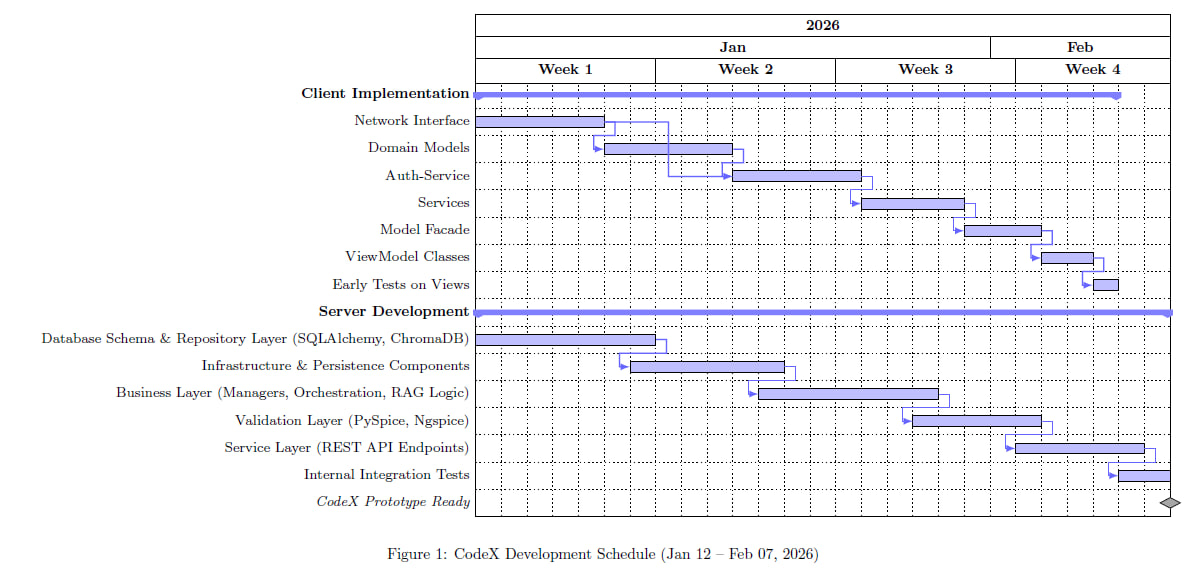
\includegraphics[width=1.1\textwidth]{figures/gannt_planned.jpg}
    \caption{Planned Project Timeline}
    \label{fig:gantt-planned}
\end{figure}

The actual implementation strayed far from this planned approach. While the general structure was followed, the linear approach could not be adhered to.
Instead, some components were developed simultaneously to get immediate feedback and to allow manual testing before a component was fully finished. \\

The changes that were made to the architecture also affected the schedule. After identifying a problem in the architecture, the already implemented parts needed to be re-adjusted to the changes. This happened several times in both the server and client.

\section{Empirical Schedule}
The empirically track the progress made on the code-base, we used data provided by the git-history of both projects. See Figure \ref{fig:empirical-client-loc} and \ref{fig:empirical-server-loc} for an overview of the Lines of Code.

\begin{figure}
    \centering
    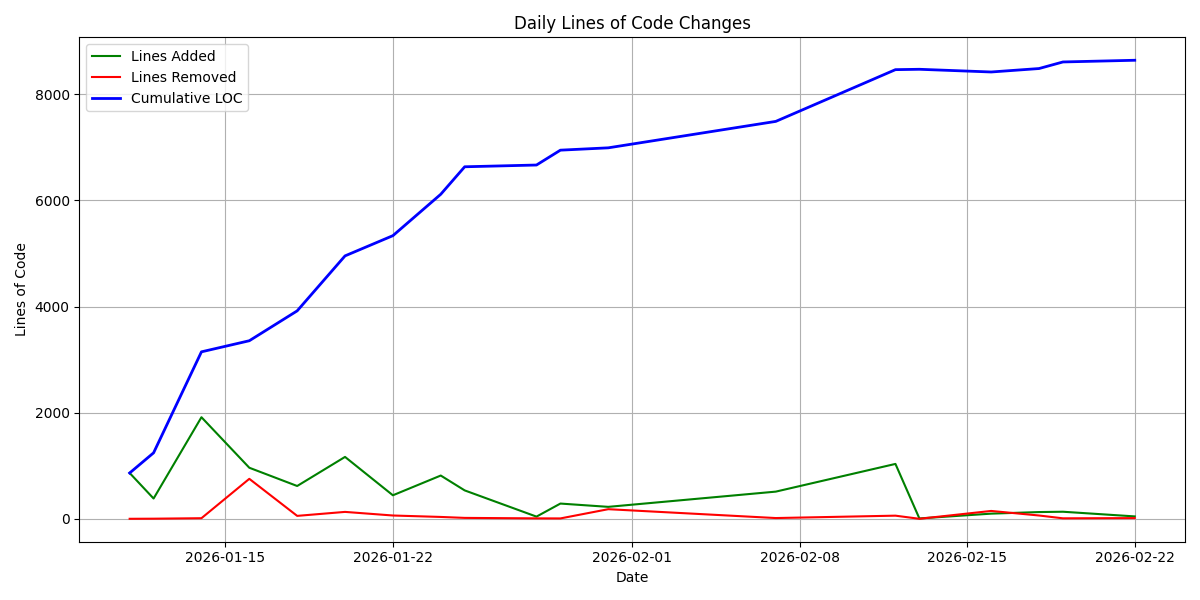
\includegraphics[width=0.8\textwidth]{figures/client_loc.png}
    \caption{Empirical Client Lines of Code}
    \label{fig:empirical-client-loc}
\end{figure}

\begin{figure}
    \centering
    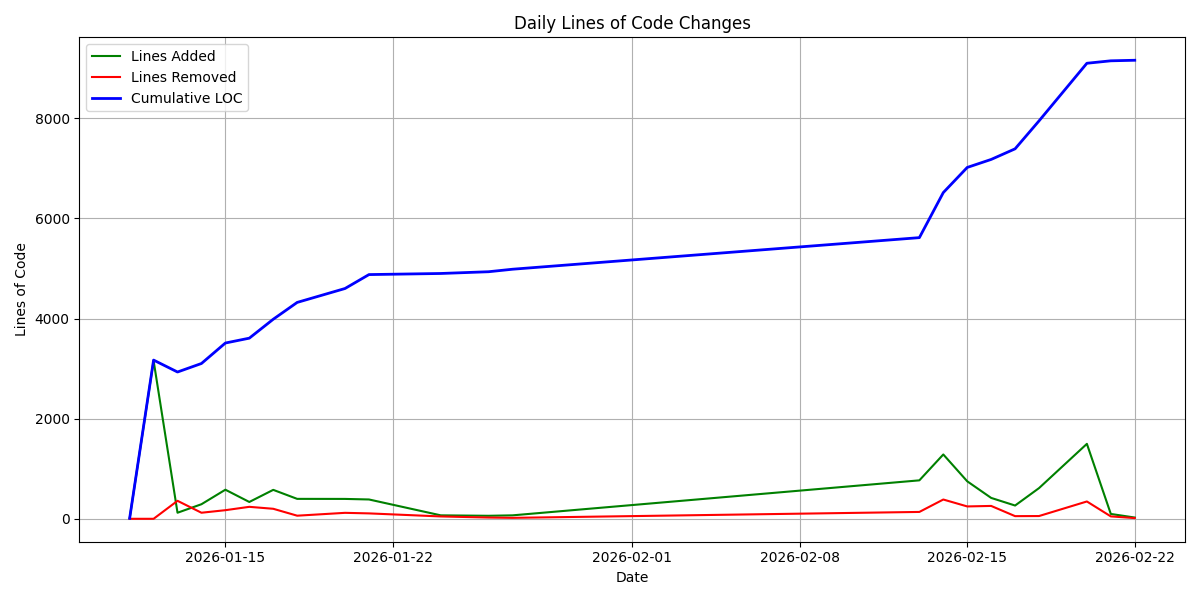
\includegraphics[width=0.8\textwidth]{figures/server_loc.png}
    \caption{Empirical Server Lines of Code}
    \label{fig:empirical-server-loc}
\end{figure}

\section{Analysis of Difficulties}
\label{subsec:analysis-delays}

The learning curve associated with the chosen technologies, especially in the context of asynchronous request handling and interactive client-side visualization, was steeper than originally estimated. Additionally, the implementation of robust error handling and validation mechanisms required more effort than planned.

Unforeseen issues, such as unexpected bugs and integration problems, as well as human factors, also had an effect on the implementation. Over the course of the project, however, the team benefited from a noticeable learning effect. As a result, later development tasks could be completed more efficiently despite the initial delays.

In some cases, delays were mitigated by parallelizing development activities. For example, client-side visualization components and server-side processing logic were partially developed in parallel once stable interfaces had been defined. Nevertheless, certain trade-offs were necessary. In particular, some optional features and a more extensive test coverage had to be deprioritized in order to meet the overall project deadline.

\subsection{Internal Communication}
\label{subsec:internal-communication}

Effective communication was a key factor in the successful implementation of the Codex project. The development team relied on a combination of digital tools and regular in-person meetings to stay coordinated. WhatsApp was used for day-to-day communication, enabling quick questions, status updates, and immediate coordination, while Discord facilitated more technical discussions, including design decisions, problem-solving, and real-time collaboration, particularly for remote team members.

Regular on-site meetings complemented the digital communication by allowing face-to-face discussions of project progress, upcoming tasks, and complex issues. This blended approach ensured that team members remained aligned and informed, with clear documentation of decisions, well-defined responsibilities, and prompt resolution of misunderstandings. Overall, this structured communication strategy contributed significantly to efficient coordination and helped the team navigate technical challenges effectively.

\section{Technical Development Environment and Infrastructure}
\label{subsec:technical-environment}

This section describes the technical development environment and infrastructure used during the implementation of the Codex project. It covers the development environments employed by the team, the tools used for implementation, as well as the version control strategy and its evolution over the course of the project.

\subsection{Integrated Development Environment}
\label{subsubsec:ide}

Within the development team, no single, unified Integrated Development Environment (IDE) was enforced.
Given the fact that IDE's are only supportive tools, every member used their own individual approach.
Namely, the following IDE's were used:

\begin{itemize}
    \item Jetbrains PyCharm
    \item Jetbrains Intellij IDEA Ultimate
    \item Jetbrains WebStorm
    \item Visual Studio Code
\end{itemize}

\subsection{Development Tools}
\label{subsubsec:dev-tools}

For backend development, no dedicated or standardized development tools were enforced beyond the selected IDEs. The project did not rely on a centralized build system, automated formatting tools, or static code analysis frameworks.

Instead, development was carried out using the built-in functionality of the respective development environments. Code structure, formatting, and quality were maintained manually by the team members according to agreed conventions.

Furthermore, no automated pipelines or integrated quality assurance tools were used during development. Dependency management and configuration were handled directly by the respectively used framework.

\subsection{Version Control}
\label{subsubsec:version-control}

Git was used as the version control system for the project. Each team member worked with an individual local repository, while a shared remote repository (for each, server and client) hosted on GitHub was used to coordinate development and integrate contributions.

From the beginning of the project, development was organized using a structured branching strategy. Separate branches were created for individual layers of the application as well as for smaller, clearly defined tasks. In most cases, a single team member was responsible for implementing and maintaining a branch.

When necessary, collaboration on a branch took place without complications. The scope of tasks was clearly defined, which prevented overlapping changes and minimized the risk of conflicts. As a result, the team did not encounter significant merge conflicts during development.

Pull requests were used to integrate completed work into the main branch. Since responsibilities and task boundaries were well coordinated, merges were performed in a controlled and orderly manner. No fast-forward merge strategy was specifically enforced, as the existing workflow already ensured a clear and understandable project history.

Overall, the consistent branching structure and clear task allocation enabled smooth collaboration throughout the entire implementation phase.
%!TEX root = ../Implementation.tex

\chapter{Deviations from the Design Document}

This chapter describes the deviations between the originally specified architecture of the \textit{Codex} system and the architecture that was ultimately implemented. Both the server architecture and the client architecture largely preserved their fundamental structural concepts. However, during implementation, several refinements and pragmatic adaptations were introduced to improve maintainability, robustness, testability, and scalability.

The following sections present architectural adjustments and implementation-level refinements for both server and client components.

\section{System-Wide}
\subsection{Role Based Authorization}
In the implementations, the roles for \textbf{Anonymous User} and \textbf{Unverified user} were merged. 
This decision was made when looking at the users in $G_{unverified} \setminus G_{anonymous}$, that did not have any more modelled permissions that anonymous users.

\section{Server}

\subsection{Consolidation of Business Interfaces}

The original server design defined a highly granular Business Layer consisting of several explicit interfaces, including \texttt{IInferenceManager}, \texttt{IAuthManager}, \texttt{IUserInfoManager}, \texttt{ISystemManager}, and \texttt{IPromptManager}. Each interface was specified as an independent contract with clearly separated responsibilities.

During implementation, the system evolved toward a domain-oriented structure. Instead of strictly mirroring each UML interface as an individual component, business logic was grouped by cohesive domains such as authentication, conversations, quota management, and analytics.

\textbf{Motivation.}  
This consolidation improved cohesion and reduced unnecessary fragmentation. Closely related responsibilities were maintained within unified domain modules, simplifying navigation and maintainability without violating the layered architecture.

\subsection{Distributed Inference Orchestration}

The original design introduced \texttt{IInferenceManager} as a central orchestration engine responsible for semantic retrieval, prompt construction, AI interaction, validation, and conversation state management.

In the implemented system, these responsibilities were distributed across collaborating components:
\begin{itemize}
    \item Conversation management in the business layer,
    \item Semantic retrieval in the persistence layer,
    \item AI interaction via a dedicated AI client,
    \item Validation logic in specialized utilities.
\end{itemize}

\textbf{Motivation.}  
Distributing orchestration responsibilities prevents the emergence of a monolithic component and enhances modularity. While deviating from the concept of a single inference interface, this structure improves testability and separation of concerns.

\subsection{Adaptation of the Repository Abstraction}

The design specified a large \texttt{IEntityRepository} interface aggregating all data-access responsibilities.

In practice, the persistence layer was implemented with structured repository abstractions organized by functional domains. Rather than relying on a single monolithic interface, responsibilities were logically decomposed while preserving abstraction boundaries between business and persistence layers.

\textbf{Motivation.}  
This decomposition improves cohesion and reduces coupling. It represents a structural refinement that strengthens maintainability without changing the conceptual data access abstraction.

\subsection{Server: Security as Service-Level Dependency}

Originally, authentication and token lifecycle logic were exclusively assigned to \texttt{IAuthManager} in the business layer.

In the implemented architecture, JWT validation and role checks are provided as reusable service-layer dependencies injected directly into API endpoints.

\textbf{Motivation.}  
Integrating security at the API layer improves clarity and reduces repetitive validation logic inside business managers. The separation between authentication logic and endpoint-level enforcement becomes clearer and more declarative.

\subsection{Centralized Error Translation}

The original design defined domain-specific exceptions but did not specify a centralized HTTP error mapping strategy.

The implemented architecture introduces a unified error-handling component at the service layer, mapping internal exceptions to consistent HTTP responses.

\textbf{Motivation.}  
Centralized error translation improves API consistency and clearly separates internal error semantics from external response contracts.

\section{Client}

\subsection{Strengthening of Authentication Architecture}

The original \texttt{AuthService} defined reactive account state and explicit login and refresh methods.

During implementation, additional internal mechanisms were introduced:
\begin{itemize}
    \item Separation of access and refresh tokens,
    \item Introduction of a \texttt{TokenStore} abstraction,
    \item Automatic refresh during application initialization,
    \item Centralized concurrency control for refresh operations.
\end{itemize}

\textbf{Motivation.}  
These refinements improve session persistence, testability, and user experience without altering the external service interface.

\subsection{DTO Formalization and Mapping Layer}

The original design intentionally separated DTOs and Domain-Models. This concept was retained and formalized further during implementation through dedicated DTO directories and mapping utilities.

\textbf{Motivation.}  
This strict separation isolates backend contract changes to the mapping layer and protects domain logic and ViewModels from structural API changes.

\section{Overall Assessment}

Despite structural deviations from the exact interface definitions in the design document, both server and client architectures remain faithful to the original conceptual model:
\begin{itemize}
    \item Clear layered server architecture,
    \item Consistent application of dependency inversion,
    \item Network abstraction on the client,
    \item Separation of DTOs and Domain-Models,
    \item Reactive services as single sources of truth,
    \item ViewModel-based UI encapsulation.
\end{itemize}

The deviations introduced during implementation primarily represent pragmatic refinements aimed at improving maintainability, robustness, modularity, and production readiness.

Rather than weakening the architectural integrity of Codex, these adjustments resulted in a more cohesive, scalable, and resilient system while preserving the conceptual foundations established in the original design document.

\chapter{Artifacts}
The final result of the Implementation phase is a shared git-repository for the server and client.

\section{Structure}
The repository consists of three files.
\begin{itemize}
    \item \textit{server/}: Directory containing a fastapi-project for the server
    \item \textit{client/}: Directory containing an angular-project for the client
\end{itemize}

\section{Usage}
To use the generated artifacts, the following needs to be done:
\begin{enumerate}
    \item Build image for the server
    \item Build image for the client
    \item Configure the external services
    \item Start a server container
    \item Start a client container
\end{enumerate}

The following section portrays an example usage using docker-compose.

\subsection{Example Usage}
\subsection{Step 1: Building the images}
To build the images, following sequence of commands can be used on a unix-like system:
\begin{minted}[gobble=4,frame=single,linenos]{shell}
    # Building the client image
    user@host:~$ cd client
    user@host:~$ docker build . -t codex/client

    # Building the server image
    user@host:~$ cd ./../server
    user@host:~$ docker build . -t codex/server
\end{minted}

After this, the local docker system contains the images \texttt{codex/client} and \texttt{codex/client}.

\subsection{Step 2: Configuring the external services}

The following shows a \texttt{docker-compose.yml} file that declares a PostgreSQL database and a ChromaDB instance.

\begin{minted}[gobble=4,frame=single,linenos]{yaml}
    services:
        db:
            image: postgres:16-alpine
            environment:
                POSTGRES_DB: codex
                POSTGRES_USER: codex_user
                POSTGRES_PASSWORD: codex_password
            ports:
                - "5432:5432"
            volumes:
                - ./data/postgres:/var/lib/postgresql/data

        chroma:
            image: chromadb/chroma:latest
            ports:
                - "8001:8000"
            environment:
                IS_PERSISTENT: "TRUE"
                PERSIST_DIRECTORY: "/chroma/data"
                CHROMA_DB_IMPL: duckdb+parquet
            volumes:
                - ./data/chroma:/data
\end{minted}

\subsection{Step 3: Configuring the server}

The following shows the service configuration for the server in the same \texttt{docker-compose.yml} file as above.

\begin{minted}[gobble=4,frame=single,linenos]{yaml}
      server:
        image: codex/server
        depends_on:
            - db
            - chroma
        ports:
            - "8000:8000"
        volumes:
            - ./data/documents:/app/docs
            - ./data/pictures:/app/pictures
        environment:
            APP_MAIL: <mail>
            MAIL_PASSWORD: <mail-password>
            APP_MAIL_SMTP_SERVER: <smtp-host>
            APP_MAIL_SMTP_PORT: <smtp-port>
            JWT_SECRET: example-secret-here
            CLIENT_SECRET: <google-client-secret-here>
            CLIENT_ID: <google-client-id-here>
            CLIENT_BASE_URL: <url-of-client>
            DATABASE_URL: "postgresql://codex_user:codex_password@db:5432/codex"
            CHROMA_PORT: 8000
            CHROMA_HOST: chroma
            ADMIN_EMAIL: admin@example.com
            ADMIN_USERNAME: admin
            ADMIN_PASSWORD: admin
\end{minted}

\subsection{Step 4: Configuring the client}

The following shows the service configuration for the client in the same \texttt{docker-compose.yml} file as above.

\begin{minted}[gobble=4,frame=single,linenos]{yaml}
        client:
            image: codex/client
            depends_on:
                - server
            ports:
                - "8080:80"
            environment:
                SERVER_BASE_URL: <url-of-server>
                GOOGLE_CLIENT_ID: <google-client-id-here>
\end{minted}

\subsection{Step 5: Starting the containers}

To start all containers, the following bash-command is used: 

\begin{minted}[gobble=4,frame=single,linenos]{shell}
    user@host:~$ docker compose up
\end{minted}

%------Ende des Dokumentes------------------------------------------------------
\end{document}
